\section{Question 2 - \textit{word count: 869}}



\subsection{Pumped hydro storage}

Pumped hydro storage (PHS) is a mature technology which resembles conventional hydroelectric power stations.
PHS differs from conventional plants in that it has an upper and lower reservoir, as well as a pump which transports water back uphill to the upper reservoir \citep{Kocher-Oberlehner2014, ScotsRenewables2011}.
PHS typically operates on a daily cycle, using surplus electricity to pump water uphill during times of low demand (e.g. at night) and discharging during times of peak demand (e.g. the UK's daily peak demand at 6~PM $\pm$ 2 hours) \citep{Mearns2018, Kocher-Oberlehner2014, ScotsRenewables2011}.
Due to its almost immediate response time in the range of 30 seconds to 2 minutes, PHS is particularly good at dealing with large fluctuations in grid demand \citep{ScotsRenewables2011, ESMStudy2010}.
PHS schemes make money from the predictable price arbitrage that exists in wholesale electricity markets \citep{Mearns2018, Strathclyde2004}.

Most PHS schemes in the UK, France and Switzerland operate alongside nuclear power plants, which produce a stable output of electricity independent of demand \citep{Mearns2018, Kocher-Oberlehner2014}.
However, PHS can also work well to compensate for the intermittent nature of renewable electricity generation (REG) from wind or solar \citep{Kocher-Oberlehner2014}.

The efficiency of a PHS scheme is considered to be between 75\% and 95\%, depending on the source.
It depends on losses due to things such as electricity conversion, friction in the conduits, pump and turbine inefficiencies.
It can also vary due to aspects such as precipitation and the duration of water storage (which can results in evaporation losses or leaks into the groundwater) \citep{WillsComment2015, Kocher-Oberlehner2014}.

\hl{``
	The rating of PHS is the highest all over the avail-able EESs, hence it is generally applied for energy manage-ment, frequency control and provision of reserve."} \citep{Chen2009}

\begin{comment}
``\textbf{How does it work?}
A pumped-storage hydroelectric power plant is a net consumer of energy but allows energy to be stored when electricity is plentiful and released for generation in times of high grid demand. Water is pumped uphill to a high reservoir when the demand, and price, for electricity is low. During hours of peak demand, when the price of electricity is high, the stored water is released through turbines to produce electric power.

``Unlike most other types of power station hydroelectric power plants can be brought online almost immediately, making them eminently suitable for dealing instantly with quite large fluctuations in grid demand."
\url{http://scotsrenewables.com/blog/distributionandstorage/pumped-storage-hydro-in-scotland/}

``Pumped storage is an extremely flexible method of storing large quantities of potential energy and highly profitable. All four United Kingdom pumped storage schemes are owned directly or in directly by electricity supply companies, and make substantial net income from the peak energy market."
\url{http://www.esru.strath.ac.uk/EandE/Web_sites/03-04/wind/content/storage%20available.html}

``i.e. Pumped hydro storage is around 75\% efficient (depends a bit on how long you’re storing it, like if some of the water you’ve pumped up evaporates over summer, or leaks away to groundwater). Part of these losses will be offset by normal rainfall collection, just like in conventional hydropower (which may be included in some efficiency calculations to make them look better).
Ben Cruachan apparently gains ~10\% of it’s delivered power from collecting rainwater, for example."
Comment from \url{http://scotsrenewables.com/blog/distributionandstorage/pumped-storage-hydro-in-scotland/}

``Most pumped hydro storage schemes in countries like the UK, France and Switzerland operate in tandem with nuclear power where surplus (low price) electricity is used to pump and store water at night, every night, to supply power into the daily peak demand (high price) that in the UK occurs at 18:00 plus or minus 2 hours. The facilities get used every day and make money from the predictable price arbitrage that exists in wholesale electricity markets."
\url{http://euanmearns.com/coire-glas-the-raging-best-of-pumped-hydro-storage/}
\end{comment}



%%% SUBSECTION %%%

\subsection{Existing PHS schemes in Scotland}

Scotland currently has two PHS schemes: Cruachan and Foyers (see Table~\ref{tbl:existing_phs}).

% Please add the following required packages to your document preamble:
% \usepackage{booktabs}
\begin{table}[htbp]
	\caption{The key characteristics of Scotland's existing PHS schemes \citep{ESMStudy2010, Strettle2013, MacKayDavid2009, ScottishPowernd}.}
	\label{tbl:existing_phs}
	\centering
	\begin{tabular}{@{}lccccc@{}}
		\toprule
		Station & \specialcell{Head \\ (m)} & \specialcell{Capacity \\ (MW)} & Response time & \specialcell{Stored energy \\ (GWh)} & \specialcell{Annual output \\ (GWh)} \\ \midrule
		Cruachan & 360 & 440 & \begin{tabular}[c]{@{}c@{}}2 mins from stationary\\ 30 sec if spinning\end{tabular} & 7 - 10 & 705 - 885 \\
		Foyers & 175 & 300 & 2 mins from stationary & 5 - 6 & 446 - 560 \\ \midrule
		Total &  &  &  & 12 - 16 & 1151 - 1445 \\ \bottomrule
	\end{tabular}
\end{table}



\subsubsection{Cruachan}

Different figures have been found for the stored potential energy in Cruachan's reservoir, including 7~GWh \citep{Strettle2013}, 8.8~GWh \citep{ESMStudy2010} and 10~GWh \citep{MacKayDavid2009}.
It is believed that these figures depend on the system efficiencies the authors are considering.
The potential energy P\textsubscript{E} (J) can be calculated using Equation~\ref{eq:PE}, where $\rho$ is the density of water (kg/m\textsuperscript{3}), g is the gravitational constant (m/s\textsuperscript{2}), h is the head (m), V is the volume of the reservoir (m\textsuperscript{3}) and $\eta$ is the system efficiency.
Cruachan's total potential energy (disregarding efficiency) is calculated to be 9.81~GWh.
However, if you consider an efficiency of 75\%, the potential energy comes down to 7.36~GWh.
For the purpose of this exercise and to avoid overestimations of PHS capacity, we will consider a PHS efficiency of 75\%.

	\begin{equation}\label{eq:PE}
		P_E = \rho \cdot g \cdot h \cdot V \cdot \eta
	\end{equation}

Cruachan generated a total of 885~GWh of electricity in 2008 and 705~GWh in 2009 \citep{ScottishPowernd}.
Its annual output depends on the system efficiency and annual capacity factor.
Considering an efficiency of 75\%, Cruachan's capacity factors in 2008 and 2009 were respectively 26\% and 33\%.

``In normal conditions the plant runs for only short periods to meet increases in demand, but it is capable of operating
continuously for around 20 hours [before the reservoir depletes itself of water] if necessary" \citep{ScottishPowernd, Mearns2018}.
Cruachan also needs to maintain a 12~hour emergency supply in reserve \citep{Mearns2018}.



\subsubsection{Foyers}

Foyers was originally built as a hydroelectric station to power an aluminium smelter in 1896.
After the smelter closed, the facility was redeveloped as a PHS station in 1969 \citep{ScotsRenewables2011, Strathclyde2004}.
The refurbishment entailed the construction of a new power station and four kilometres of steel lined tunnelling five metres in diameter through porous rock.
New turbines and generators were installed and the transmission lines were upgraded to cope with the additional power \citep{Strathclyde2004}.

Information on Foyers' energy storage capacity and annual output were not found.
Hence, these figures in Table~\ref{tbl:existing_phs} have been estimated based on the Cruachan findings.
Foyers' stored potential energy is between 4.65~GWh (at 75\% efficiency) and 6.20~GWh (disregarding efficiency).
Considering an efficiency of 75\%, Foyers' annual output varies between 446~GWh ($CF = 26\%$) and 560~GWh ($CF = 33\%$).

\begin{comment}
\textbf{Cruachan}

``The Cruachan station on Loch Awe became fully operational in 1967  and  was the first reversible pump storage hydro system to be built in the world. Cruachan generated 885 GWh of electricity in 2008."
\url{http://scotsrenewables.com/blog/distributionandstorage/pumped-storage-hydro-in-scotland/}

``There are four 100MW Francis reversible pump turbines in the cavern.
Cruachan’s maximum output is 440MW — enough to power 225,000 homes.
It can achieve full power from shut down in two minutes, or 30 seconds if compressed air is used to start the turbine blades spinning first.
[\ldots]

``Water is pumped uphill from Loch Awe to the reservoir during periods of low energy demand (such as at night), to cope with peak demand later.

``The power station can operate continuously for 22 hours before the water in the reservoir is used. It has to maintain a 12 hour emergency supply in reserve."
\url{https://web.archive.org/web/20140426153739/http://www.engineering-timelines.com/scripts/engineeringItem.asp?id=1006}


\textbf{Foyers}

``The Foyers hydro electric scheme was originally built by the british Aluminium Company in 1896 to power an aluminium smelter and was the first large-scale commercial hydro-electric scheme in the UK. It was redeveloped to focus on pumped-storage in 1969."
\url{http://scotsrenewables.com/blog/distributionandstorage/pumped-storage-hydro-in-scotland/}

``Research showed that Foyers Pumped Storage Scheme started life as pure Hydro Electric Generation Station. Built by Alcan in 1896 to produce electricity for their aluminium smelter. The smelter closed in 1968. The Hydro scheme was purchased by Scottish Power who re-designed it. The original Hydro Scheme consisted of six 500Kw turbines [\ldots]
The original power station was retained and re-furbished with a one single 5Mw Turbine running as a pure hydro-electric generating station, it runs on average 10.6 hours per day.

``The construction of Foyers Pumped Storage Scheme entailed building a new Power Station adjacent to the existing Hydro Station. Four Kilometres of tunnelling 5 metres in diameter required to be driven through porous rock. The tunnels then had to be steel lined. Together with new turbines and generators, transmission lines were upgraded in order to handle the additional power.

``As a pumped storage system it generates 300Mw from two 150Mw machines. During the day the machines are kept on spinning reserve ready to meet periods of peak demand, the response time is in the order of 15 seconds. Spinning reserve requires the machines to rotate in synchronisation with the National Grid frequency. Power to keep the machines in this state of readiness, is drawn from the 5Mw adjacent hydro station.

``The cost of the power absorbed in maintaining spinning reserve is paid for by the utility requiring peak load electricity, this spinning reserve power is charged at a premium rate above normal grid prices. Peak load electricity can command prices in the thousands of pounds per Mw/hr all be it for short bursts of power at any given time. On average a pumped storage scheme may well have in excess of ten thousand stop -starts in a year.

``[\ldots]The investment in Foyers described above suggests that it may be both feasible and profitable to upgrade and refurbish other existing hydro schemes."
\url{http://www.esru.strath.ac.uk/EandE/Web_sites/03-04/wind/content/storage%20available.html}
\end{comment}



%%% SUBSECTION %%%

\subsection{Potential for additional PHS in Scotland}

\hl{``The major drawback of PHS lies in the scarcity of avail-able sites for two large reservoirs and one or two dams"} \citep{Chen2009}

Research shows that investments in new PHS schemes in Scotland is waning due to strong planning and environmental opposition and a lack of suitable green sites \citep{Strathclyde2004, ScotsRenewables2011, Chen2009}.
However, Scotland has multiple conventional hydroelectric power stations which, like Foyers, could be redeveloped as PHS facilities \citep{Strathclyde2004, MacKayDavid2009}.
Such redevelopments have proven to be popular and economically attractive in Europe since the costs of dams are avoided \citep{ESMStudy2010}.
Figure~\ref{fig:map_potential_PHS} shows 13 locations in Scotland with potential for PHS, most of which already have a hydroelectric facility.

\begin{figure}[htbp]
	\centering
	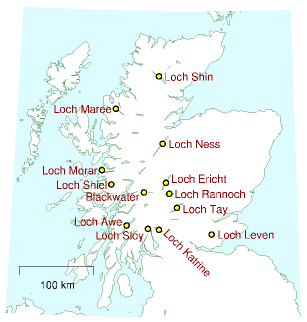
\includegraphics[width=.5\textwidth]{figures/map_potential_PHS.png}
	\rule{\textwidth}{0.5pt} % use line???
	\caption{Lochs in Scotland with potential for PHS \citep{MacKayDavid2009}.}
	\label{fig:map_potential_PHS}
\end{figure}

An example of a suitable site with an existing hydroelectric facility would use Loch Sloy as its upper reservoir and Loch Lomond as its lower reservoir \citep{MacKayDavid2009, Strathclyde2004}.
Loch Sloy already has an energy storage capacity of 20~GWh with a height difference of 270~m above Loch Lomond.
If Loch Sloy's dam were raised by another 40~m then the energy storage capacity could be raised to 40~GWh.
``The water level in Loch Lomond would change by at most 0.8~m during a cycle.
This is less than the normal range of annual water level variations of Loch Lomond (2~m)." \citep[p.~193]{MacKayDavid2009}

\begin{comment}
\textbf{Loch Sloy}

``Loch Sloy was built to provide power for the Glasgow area to meet peak electricity demand.

``[\ldots]
As previous stated Loch Sloy Hydro Scheme was built in 1948 as a peak demand station for the Glasgow area. \hl{Being close to a major city and the grid it was decided to investigate the potential for conversion to Pumped Storage. The reason being that the top reservoir Loch Sloy exists, therefore no civil engineering costs would be incurred in new dam construction. Pumped storage requires that the turbine/pumps are below the minimum water level in the lower reservoir, in this case Loch Lomond. A new power station and tunnels would require to be excavated inside Ben Vorlich.} Research in the North of Scotland Hydro-Electric annual reports uncovered the original design criteria shown below.

``Output initially 120Mw

Output now 190Mw

Annual output 130Gw hours

Top dam storage capacity 15.5\% of gross annual output.

Annual output x percentage storage capacity/365 = daily storage capacity

``Answer 20.4 GWh pumped storage capacity"
\url{http://www.esru.strath.ac.uk/EandE/Web_sites/03-04/wind/content/storage%20available.html}

	``It is also to submit to Scottish Ministers an application for consent to develop a 60MW pumped storage scheme at its existing Sloy hydro electric power station at Loch Lomond, \hl{allowing it to produce an additional 100GWh (gigawatt hours) of electricity in a typical year to help meet peak demand}."
	\url{http://scotsrenewables.com/blog/distributionandstorage/pumped-storage-hydro-in-scotland/}

	``\hl{A smaller 60 MW scheme is proposed for the existing Loch Sloy} natural flow hydro
	scheme."
	\url{https://www.webarchive.org.uk/wayback/archive/20170113164907/http://www.gov.scot/Publications/2010/10/28091356/14}

	``Pumped-storage facilities holding significantly more energy than Dinorwig
	could be built in Scotland by upgrading existing hydroelectric facilities.
	Scanning a map of Scotland, one candidate location would use
	Loch Sloy as its upper lake and Loch Lomond as its lower lake. There is
	already a small hydroelectric power station linking these lakes.
	\hl{The height difference between Loch Sloy and Loch Lomond is about 270 m. Sloy's 	area is about 1.5 km2, and it can already store an energy of 20 GWh. If	Loch Sloy's dam were raised by another 40 m then the extra energy that
	could be stored would be about 40 GWh. The water level in Loch Lomond	would change by at most 0.8 m during a cycle. This is less than the normal	range of annual water level variations of Loch Lomond (2 m).}

	``\hl{Figure 26.10 shows 13 locations in Scotland with potential for pumped}
	storage. (Most of them already have a hydroelectric facility.) If ten of these
	had the same potential as I just estimated for Loch Sloy, then we could
	store 400 GWh – one third of the total of 1200 GWh that we were aiming
	for."
	\url{https://www.withouthotair.com/c26/page_193.shtml}
\end{comment}

% There are currently two PHS sites that are planned for construction (Coire Glas - Phase~I and Glenmuckloch) and another that has been proposed (Red John Pumped Storage).

Table~\ref{tbl:potential_phs} presents the power and energy storage of potential and operational PHS schemes in Scotland, including two that are planned for construction and another that has been proposed.
Scotland has potential to store well over one week's worth of power and energy demand (1.43~GW/ 240~GWh) that was calculated in Question~1.
However, the necessary power rating of 3.43~GW to meet the peak power demand exceeds the total power potential in Table~\ref{tbl:potential_phs}.
To compensate for this, additional dispatchable power or other forms of energy storage should be considered.

% Please add the following required packages to your document preamble:
% \usepackage{booktabs}
% \usepackage{multirow}
\begin{table}[H]
	\caption{The power and energy capacity of potential and operational PHS schemes in Scotland \citep{Scotsman2018, SSE2005, SSEnd, MacKayDavid2009, Strathclyde2004, BEIS2018PlanningDatabase, Mearns2018}.}
	\label{tbl:potential_phs}
	\centering
	\begin{tabular}{@{}llrr@{}}
		\toprule
		Status & Station & Power (MW) & Energy storage capacity (GWh) \\ \midrule
		\multirow{9}{*}{\begin{tabular}[c]{@{}l@{}}Existing\\ hydroelectric\end{tabular}} & Errochty & 75.0 & 16.0 \\
		& Luichart & 2.6 & 38.0 \\
		& Clunie & 61.0 & 40.0 \\
		& Rannoch & 1.4 & 41.0 \\
		& Fasnakyle & 7.5 & 78.0 \\
		& Tummel & 34.0 & 38.0 \\
		& Invergarry & 20.0 & 41.0 \\
		& Quoich & 18.0 & 27.0 \\
		& Sloy & 190.0 & 20.0 or 40.0 \\
		&  & \multicolumn{1}{l}{} & \multicolumn{1}{l}{} \\
		Proposed PHS & Red John Pumped Storage & 499.0 & 2.4 \\
		&  & \multicolumn{1}{l}{} & \multicolumn{1}{l}{} \\
		\multirow{2}{*}{Planned PHS} & Coire Glas - Phase I & 600.0 or 1500.0 & 30.0 \\
		& Glenmuckloch & 400.0 & Unknown \\
		&  &  &  \\
		\multirow{2}{*}{Operational PHS} & Cruachan & 440.0 & 7.4 \\
		& Foyers & 300.0 & 4.7 \\ \midrule
		Total &  & 2,048.5 or 2,948.5 & $>$ 363.5 or 383.5 \\ \bottomrule
	\end{tabular}
\end{table}

\begin{comment}
``Initially sites for new build were investigated.
It became apparent that any new build on the scale required would meet \hl{strong planning and environmental opposition}."
\url{http://www.esru.strath.ac.uk/EandE/Web_sites/03-04/wind/content/storage%20available.html}

``\hl{Sites for any further pumped storage schemes are in scarce supply and likely to attract a lot of opposition from environmental groups}. Proposals have been mooted for seawater pumped storage hydro and underground pumped storage schemes, but the costs could prove prohiiibitive. For the immediate future it looks as though pumped storage may only be able to meet between a third and a half of Scotland’s future energy storage needs."
\url{http://scotsrenewables.com/blog/distributionandstorage/pumped-storage-hydro-in-scotland/}

``\hl{Installing pump-back systems on existing hydro-electric facilities. This was identified as a
popular trend in Europe as many of the economically attractive sites have been taken (Deane
et al 2010). The costs of dams are avoided. In Scotland there are likely to exist a number of
opportunities to install pump back systems on existing dams. In a study undertaken by
Strathclyde the pumped hydro potential was identified as 494 GWh from 13 sites (Sloy not
included}, as this is already being investigated). "
\url{https://www.webarchive.org.uk/wayback/archive/20170113164907/http://www.gov.scot/Publications/2010/10/28091356/14}



%%%% SUBSUBSECTION %%%%

\subsubsection{Where are the suitable sites to build PHS in Scotland?}


This section will analyse \textbf{\hl{two or three}} potential sites.


\newpage
\textbf{Coire Glas}

The 600~MW/ 30~GWh PHS scheme at Coire Glas was granted planning approval in 2013, yet construction has still not begun \citep{Mearns2018, ESMStudy2010}.
\hl{Why?}
SSE submitted a proposal in 2017 to increase Coire Glas' capacity from 600~MW to 1,500~MW \citep{Mearns2018, SSEnd}.
\end{comment}

\begin{comment}
\hl{``Back in December 2013 Scottish and Southern Energy PLC (SSE) was granted planning approval for the 600 MW / 30 GWh pumped hydro storage (PHS) scheme at Coire Glas, northern Scotland.
[\ldots] Almost 5 years on, and work on the scheme has not yet begun.
[\ldots] SSE have recently submitted an application to change the plan from 600 MW (puny) to a more raging 1500 MW  beast (see link). This may move the scheme towards profitability but it also moves the specification in the exact opposite direction of that required for storing variable wind power."}
\url{http://euanmearns.com/coire-glas-the-raging-best-of-pumped-hydro-storage/}
\end{comment}



%%% SUBSECTION %%%

\subsection{Costs}

The capital costs of PHS plants can range from as low as \$500/kWh to
\$8000/kWh. In terms of capacity, this means between the range of \$1000/kW and
\$6000/kW. While the Capital Cost is a long term investment with typical
payback time of 20 to 40 years, it is worthy to consider that the typical
lifetime of a PHS plant is over \hl{100 years}. The large variations in
\hl{kWh} and payback time correlates with variations arising from differences
in site design, labour costs and amount and type of materials required; this is
generally the same with conventional Hydropower plants
\citep{Kocher-Oberlehner2014}.

PHS is well understood and cost effective since it has existed for a
while\citep{ESMStudy2010, Ramirez2016}, this means that it has a high storage
period and high efficiency with a low capital cost per unit of energy.  In
fact, the cost per cycle kWh of PHS is one of the lowest of all the EES
technologies \citep{Chen2009}.

% AIM: Costs to build the required electricity storage using PHS only

%`` Capital Costs of PHS plants have a large variation and range from as low as
%500 to as high as 8000 \$/kWh. Or, in terms of capacity, they range between
%1000 and 6000 \$/kW. They are long term investments with typical pay-back times
%of 20 to 40 years, but also with a life time of over 100 years. The large
%variations come from differences in site, design, labour costs and how much and
%which materials are necessary, very similar to conventional Hydropower plants."
%\citep{Kocher-Oberlehner2014}

%``PHS is a mature technology with large volume, long storage period, high efficiency and relatively low capital cost per unit of energy." \citep{Chen2009}
%
%Cost effective \citep{ESMStudy2010, Ramirez2016}
%``The costs per cycle kWh of PHS and CAES are among
%the lowest among all the EES technologies," \citep{Chen2009}

%high cost for capacity \citep{Sterner2017}

PHS plants tend to be operational for a duration of 50 to 100 years with a high
capital cost and low operational and maintenance (O\&M) cost. There is no fixed
or standard project cost for PHS systems because this cost very much depends on
the intended site with quoted costs varying from 450 - 2500~\euro{}/kW.  The
capital cost is not solely dependent on the installed power but also on the
energy storage (reservoirs) and power rating at the given site.  Being a mature
technology, PHS's capital cost is not expected to change substantially in the
future \citep{Zach2012}.

%``Typically, PHS plants are characterised by long asset life (typically 50 – 100 years), high capital
%cost and low operation and maintenance (O\&M) cost. Project costs for PHS systems are very site
%specific with some quoted costs varying from of 450 – 2500 euros/kW. Additionally capital costs
%depend not only on the installed power but also on the energy storage (reservoirs) and power
%rating at any given site. Since PHS is a mature technology, its capital cost is not expected to
%change substantially in the future."
%\citep{Zach2012}
%Lifetime: 40-60 years \citep{Chen2009}

Constructing and deploying a PHS entails some major constraints. There is an
approximate lead in time of 10 years and a high cost in the realm of hundreds
to thousands of millions of US dollars. There are also environmental issues
such as removing trees and vegetation from the large amounts of land required
by the reservoir. Other considerations include the length of the waterways;
long waterways are costly and result in higher hydraulic losses. There is also
the transmission distance to demand, the shorter this distance the better
because this simultaneously reduces transmission integration cost and
transmission losses. A scheme located in the vicinity of the generation centres
and near the main national grid is ideal \citep{Louwinger2008}.

\begin{table}[htbp]
\begin{tabular}{@{}lll@{}}
\toprule
Design scenario & Plant size & Capital cost \\ \midrule
1week storage & 1.43 GW/240GW & £0.5b - £146.2b \\
Meet peak demand & 3.43 GW & £1.3b - £15.7b \\ \bottomrule
\end{tabular}
\end{table}

%\textbf{Construction}
%
%Capital costs \citep{Chen2009}:
%\$ per kW: 600-2000.
%\$ per kWh: 5-100
%
%\hl{``A long lead time (typically ?10 years) and a high cost (typically
%hundreds to thousands of million US dollars) for con-struction and
%environmental issues (e.g. removing trees and vegetation from the large amounts
%of land prior to the res-ervoir being flooded) [45,46] are the other three
%major con-straints in the deployment of PHS."} \citep{Chen2009}

%A larger storage volume costs more to construct, but increases
%the utilisation of the scheme and reduces the operating cost of
%other more expensive plant. cite \citep{Louwinger2008}

%Long waterways are costly and result in higher hydraulic losses. cite \citep{Louwinger2008}

%Transmission distance to demand - the closer the better.
%``\textbf{Location from main demand and generating
%	centres:} To avoid excessive transmission integration
%cost and transmission losses, it was important that the
%scheme was located in the vicinity of the generating
%centres and near the main national grid."
%cite \citep{Louwinger2008}


\begin{comment}
``Economic Conclusions
\hl{Pumped storage is the most cost effective of the large scale energy storage technologies that can be
used in Scotland.} A high level assessment of pumped storage economics suggests that new pumped
storage would be more expensive than constraining renewable energy generation off the network.
This assessment does not include other potential revenues that a pumped storage device may be able
to access but these are unlikely to revise the economic case radically. The conclusion reinforces the
view that accommodating the forecast generating plant mix under the highest renewable energy
Scenarios \hl{will require a wide range of solutions of which the various demand side response measures
enabled by the smart grid and smart meters will be an important and cost effective component.}"
\url{https://www.webarchive.org.uk/wayback/archive/20170113164907/http://www.gov.scot/Publications/2010/10/28091356/14}

``\textbf{Reservoir capacity}
A
larger storage volume costs more to construct, but increases
the utilisation of the scheme and reduces the operating cost of
other more expensive plant.

``\textbf{Waterways}
T h e h o r i z o n tal di s tan c e be twe e n t h e uppe r
a n d l owe r r e s e r v o i r i s n o rma l l y l imi t e d t o
6000 m. Long waterways are costly and result in higher
hydraulic losses.

``\textbf{Location from main demand and generating
centres:} To avoid excessive transmission integration
cost and transmission losses, it was important that the
scheme was located in the vicinity of the generating
centres and near the main national grid."
Case study of Ingula and Lima pumped storage schemes
\end{comment}
